\chapter{Introduction}

\subsection{Problem Context}
	Astronomy is by nature an observational, data-driven science. During the last few decades the field was transformed by technology with software and databases becoming an integral part of data gathering and analysis. As the sophistication of observational equipment has improved the volume of observational data available to researchers has increased. The ASKAP\footnote{\url{http://www.atnf.csiro.au/SKA/}} telescope array under construction in Western Australia will produce a gigabyte of processed data per second . A topic of growing interest has been to automate the analysis of these large data volumes. The subject of this research is to develop algorithms for use in an automatic data analysis pipeline for detecting astronomical transient events as part of the VAST\footnote{\url{http://www.physics.usyd.edu.au/sifa/vast/index.php}} project.
	\subsection{Transients and Time Series}
	An astronomical transient event is a structural change in the observation of a stellar object such as a star or galaxy, referred to as \emph{sources} by astronomers. These observations take the form of \emph{time series}, or to astronomers, \emph{light curves}. Time series represent the intensity of an observed source in potentially multiple frequencies over some time indices. An explicit definition for time series is:
	\begin{center}
	\begin{math}
		\{(t_i, \mathbf{x}_{i}) \quad i \in \{t_{1} \ldots t_{D}\} \subset \mathbb{R} \quad \mathbf{x}_{i} \in \mathbb{R}^{D} \}
	\end{math}
	\end{center}
	a mapping from unique time indices $t_{i}$ to a $D$ dimensional vector $\mathbf{x}_{i}$. The $t_{i}$ values may represent any real unit of time - seconds, days, years. The sequence of increasing $t_{i}$ is not necessarily evenly distributed. A typical astronomical time series we are looking for is a supernova. A supernova occurs when very large stars reach the end of their life cycle resulting in a catastrophic explosion. These explosions release large amounts of radiation that can be detected from great distances.
	\begin{figure}[ht!]
	\centering
	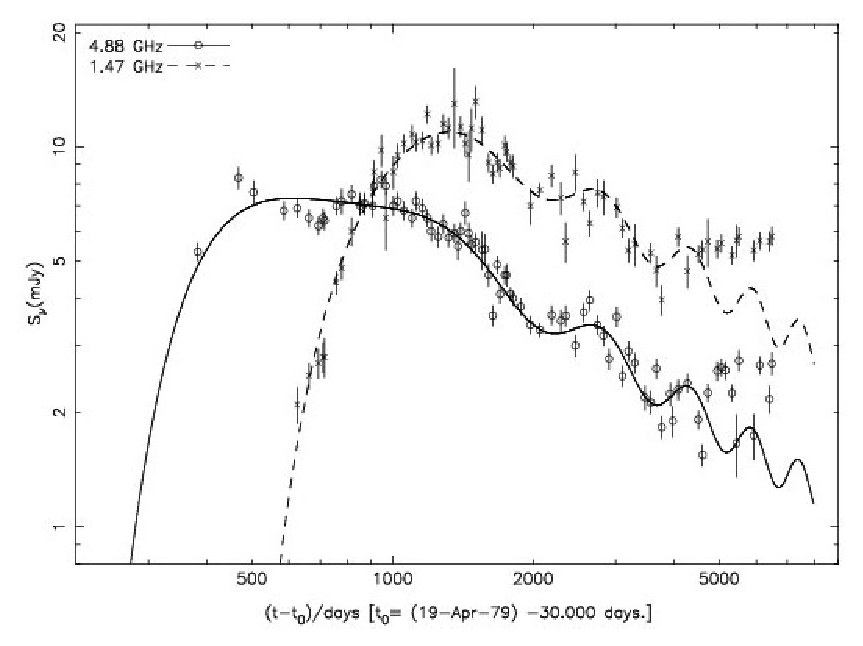
\includegraphics[width=120mm]{/Users/peter/honors/thesis/introduction/images/supernova.eps}
	\caption{Supernova light curve. The height of the observations on the y-axis indicates the observed intensity at the given time position}
	\end{figure}
	Variability in astronomical time series is not always intrinsic to the source, that is, the result of some change in the source itself such as in a supernova event. Some scintillation will result from the light interacting with the interstellar medium on its journey to earth. This is called extrinsic variation and will complicate the process of analysing the time series.
	\subsection{The Problem}
	The precise problem to be explored in this research is the development of an algorithm for the classification of streaming time series data. The algorithm will receive data every 5 seconds. At each time step any new transients will be reported and along with what class they belong to with a measure of confidence.
		\begin{itemize}
		\item Extreme scattering events (ESEs) \footnote{\url{http://ese.nrl.navy.mil/}}
		\item Gamma ray bursts \footnote{\url{http://imagine.gsfc.nasa.gov/docs/science/know_l1/bursts.html}}
		\item Supernovae
		\item X-ray binaries \footnote{\url{http://imagine.gsfc.nasa.gov/docs/science/know_l1/binary_stars.html}}
		\item Intraday variable stars
	\end{itemize}
	It is possible that a transient may belong to an undetermined class and this also needs to be taken into account. The detection of transients should be done as early as possible but should not have too many false positives.
	
	\subsection{Time Series Analysis}
	This problem is primarily one of \emph{time series analysis}. Fortunately, in recent years this field has received a lot of attention in various domains: speech recognition \citep{sakoe1978dynamic}, handwriting analysis \citep{bahlmann2002online}, even image outlines can be represented as time series and classified \citep{ye2009time}. However, the well-developed techniques from these other areas do not extend immediately to our astronomical data. The table below outlines the most serious difficulties inherent to this task.
	\vspace{10pt}
	\begin{table*}[h!]

	\centering
	$\begin{array}{lp{0.7\textwidth}}
		\textbf{incompleteness} & Data arrives as a stream, and classification must be done without full knowledge of the curve structure. Most developed techniques assume full structure data is available. \vspace{10pt} \\
		\textbf{distortions} & Astronomical time series have distortions in terms of amplitude scaling, time warping, noise and missing data. \vspace{10pt} \\
		\textbf{precision} & Classifications must have very high precision. Too many false positives will waste astronomer time and make the system useless. \vspace{10pt} \\
		\textbf{real-time} & There are very large data volumes arriving in a stream - 1 GB/s, so classification must be time and space efficient and at least near-real time. \vspace{10pt} \\ 
		\textbf{redundant} & Most data is not relevant to event detection. The start and end of interesting structures must also be determined by the program. \vspace{10pt} \\
		\textbf{periodic} & Some data will come from periodic sources and this will confuse algorithms searching for `one-off' events. Periodic time series may need to be identified and handled separately.
	\end{array}$
	\end{table*}
	
	This set of problems is not trivial, and no individual piece of research at present addresses them all. Literature from several domains: machine learning, time series analysis (in astronomy and other fields) and statistics is reviewed and discussed in the following sections with the aim of addressing these issues.
		
%	\begin{enumerate}
%		\item The data arrives in a stream, not as a full structure. Classification is needed without complete light curve data. Most developed techniques assume the entire curve is available at classification time.
%		\item Astronomical time series have distortions in terms of amplitude scaling, time stretching, noise and missing data
%		\item The classification must be very high precision so as not to waste astronomer time
%		\item There are very large data volumes - 1 GB/s so classification has to be efficient in space and time complexity
%		\item Most of the received data is not relevant to event detection - the start and end of interesting structures must also be determined by the program
%	\end{enumerate}

\subsection{Coping with Distortions in Astronomical Time Series}
	Below is a list of subproblems associated with the issue of \textbf{distortions} in our astronomical time series.
	\begin{itemize}
		\item \textbf{noisy observations}. It can be assumed that every point in a light curve has added noise. For simplicity this noise is assumed to be gaussian distributed which is a reasonable approximation of real conditions in astronomical data.
		\item \textbf{amplitude scaling} - the same astronomical event will have a different intensity when observed at different distances
		\item \textbf{missing data} - streaming data is not continuous. This may be due to bad weather or shared telescope responsibilities.
		\item \textbf{time warping} - events may have different durations or unfold slightly differently, but still have very similar structures
	\end{itemize}
	The section outlines some of the methods developed to remedy these issues both in astronomical data mining and from other areas.
	
